%%%%%%%%%%%%%%%%%%%%%%%%%%%%%%%%%%%%%%%%%%%%%%%%%%%%%%%%%%%%
%%

%%%%%%%%%%%%%%%%%%%%%%%%%%%%%%%%%%%%%%%%%%%%%%%%%%%%%%%%%%%%%
%% FSBI presentation on spatial stats and mixed fisheries %%%
%%%%%%%%%%%%%%%%%%%%%%%%%%%%%%%%%%%%%%%%%%%%%%%%%%%%%%%%%%%%%

\documentclass[xcolor=x11names,compress]{beamer}

%% General document %%%%%%%%%%%%%%%%%%%%%%%%%%%%%%%%%%
\usepackage[english]{babel}
\usepackage{graphicx}
\usepackage{epstopdf}
\usepackage{subcaption}
\captionsetup{compatibility=false}
\usepackage{tikz}
\usepackage[utf8]{inputenc}
\usepackage{times}
\usepackage[T1]{fontenc}
\usetikzlibrary{decorations.fractals}
%%%%%%%%%%%%%%%%%%%%%%%%%%%%%%%%%%%%%%%%%%%%%%%%%%%%%%

%% Beamer Layout %%%%%%%%%%%%%%%%%%%%%%%%%%%%%%%%%%
\useoutertheme[subsection=false,shadow]{miniframes}
\useinnertheme{default}
\usefonttheme{serif}
\usepackage{palatino}

\setbeamerfont{title like}{shape=\scshape}
\setbeamerfont{frametitle}{shape=\scshape}

\setbeamercolor*{lower separation line head}{bg=DeepSkyBlue4} 
\setbeamercolor*{normal text}{fg=black,bg=white} 
\setbeamercolor*{alerted text}{fg=red} 
\setbeamercolor*{example text}{fg=black} 
\setbeamercolor*{structure}{fg=black} 
 
\setbeamercolor*{palette tertiary}{fg=black,bg=black!10} 
\setbeamercolor*{palette quaternary}{fg=black,bg=black!10} 

\definecolor{mygreen}{cmyk}{0.82,0.11,1,0.25}
\setbeamertemplate{blocks}[rounded][shadow=false]
\addtobeamertemplate{block begin}{\pgfsetfillopacity{0.8}}{\pgfsetfillopacity{1}}
\setbeamercolor{structure}{fg=mygreen}

\renewcommand{\(}{\begin{columns}}
\renewcommand{\)}{\end{columns}}
\newcommand{\<}[1]{\begin{column}{#1}}
\renewcommand{\>}{\end{column}}

\graphicspath{{figures/}}

%%%%%%%%%%%%%%%%%%%%%%%%%%%%%%%%%%%%%%%%%%%%%%%%%%
\AtBeginSection{\frame{\sectionpage}}

 
\titlegraphic{
	\includegraphics[width = 1.5cm]{MRFC_Bubble} \hspace*{4.6cm}
	\includegraphics[width = 2.5cm]{seedcorn_logo_white_navy_bkgd}  \\
	\includegraphics[width = 2.5cm]{gmit-logo} \hspace*{1cm}
	\includegraphics[width = 2.5cm]{MARES} \hspace{1cm}
	\includegraphics[width = 2.5cm]{cefas_fish_white_dark_blue_bkgd}
	}

\begin{document}

\addtocounter{framenumber}{-1}

%%%%%%%%%%%%%%%%%%%%%%%%%%%%%%%%%%%%%%%%%%%%%%%%%%%%%%
%%%%%%%%%%%%%%%%%%%%%%%%%%%%%%%%%%%%%%%%%%%%%%%%%%%%%%
\begin{frame}
\title{Using spatio-temporal population models to inform mixed-fishery management}


\author{Paul Dolder}
\author[shortname]{Paul J. Dolder, \inst{1,2} \and 
	James Thorson \inst{3} \and 
	Cóilín Minto\inst{1}}
\vspace{-0.5cm}

\institute[shortinst]{\inst{1}Galway-Mayo Institute of Technology, Ireland
	\and \vspace{-0.2cm}
\inst{2} Centre for Environment, Fisheries and Aquaculture Science, UK \and
\vspace{-0.2cm}
\inst{3} North West Fisheries Science Center, NOAA, USA}

\date{6 July 2017 \\ FSBI Symposium, Exeter, UK}
\titlepage
\end{frame}

%%%%%%%%%%%%%%%%%%%%%%%%%%%%%%%%%%%%%%%%%%%%%%%%%%%%%%%%%%%%%%
%%%%%%%%%%%%%%%%%%%%%%%%%%%%%%%%%%%%%%%%%%%%%%%%%%%%%%%%%%%%%%

%%%%%%%%%%%%%%%%%%%%%%%%%%%%%%%%%%%%%%%%%%%%%%%%%%%%%%
%%%%%%%%%%%%%%%%%%%%%%%%%%%%%%%%%%%%%%%%%%%%%%%%%%%%%%
\begin{frame}
\tableofcontents
\end{frame}

\section{Background}
\subsection{Blah}
\begin{frame}{Scene setting}

	\begin{itemize}
		\item Most of the worlds fisheries are mixed-fisheries (i.e more
			than one species together).
		\item Fish populations are heterogeneously distributed in space
			and time.
		\item Problem for fisheries management if...
		\item Increased interest is spatio-temporal avoidance and
			dynamics and the fisheries
	\end{itemize}
	
\end{frame}

\begin{frame}{Motive}
	\begin{itemize}
		\item Want to understand how space can be used to separate
			catches in highly mixed fisheries.
		\item Developments in geostatistical methods for analysing
			catch data which is often...problems 
		\item Provide insight into how far spatial measures and
			avoidance can go to improving sustainability of mixed
			fisheries.
	\end{itemize}
	
	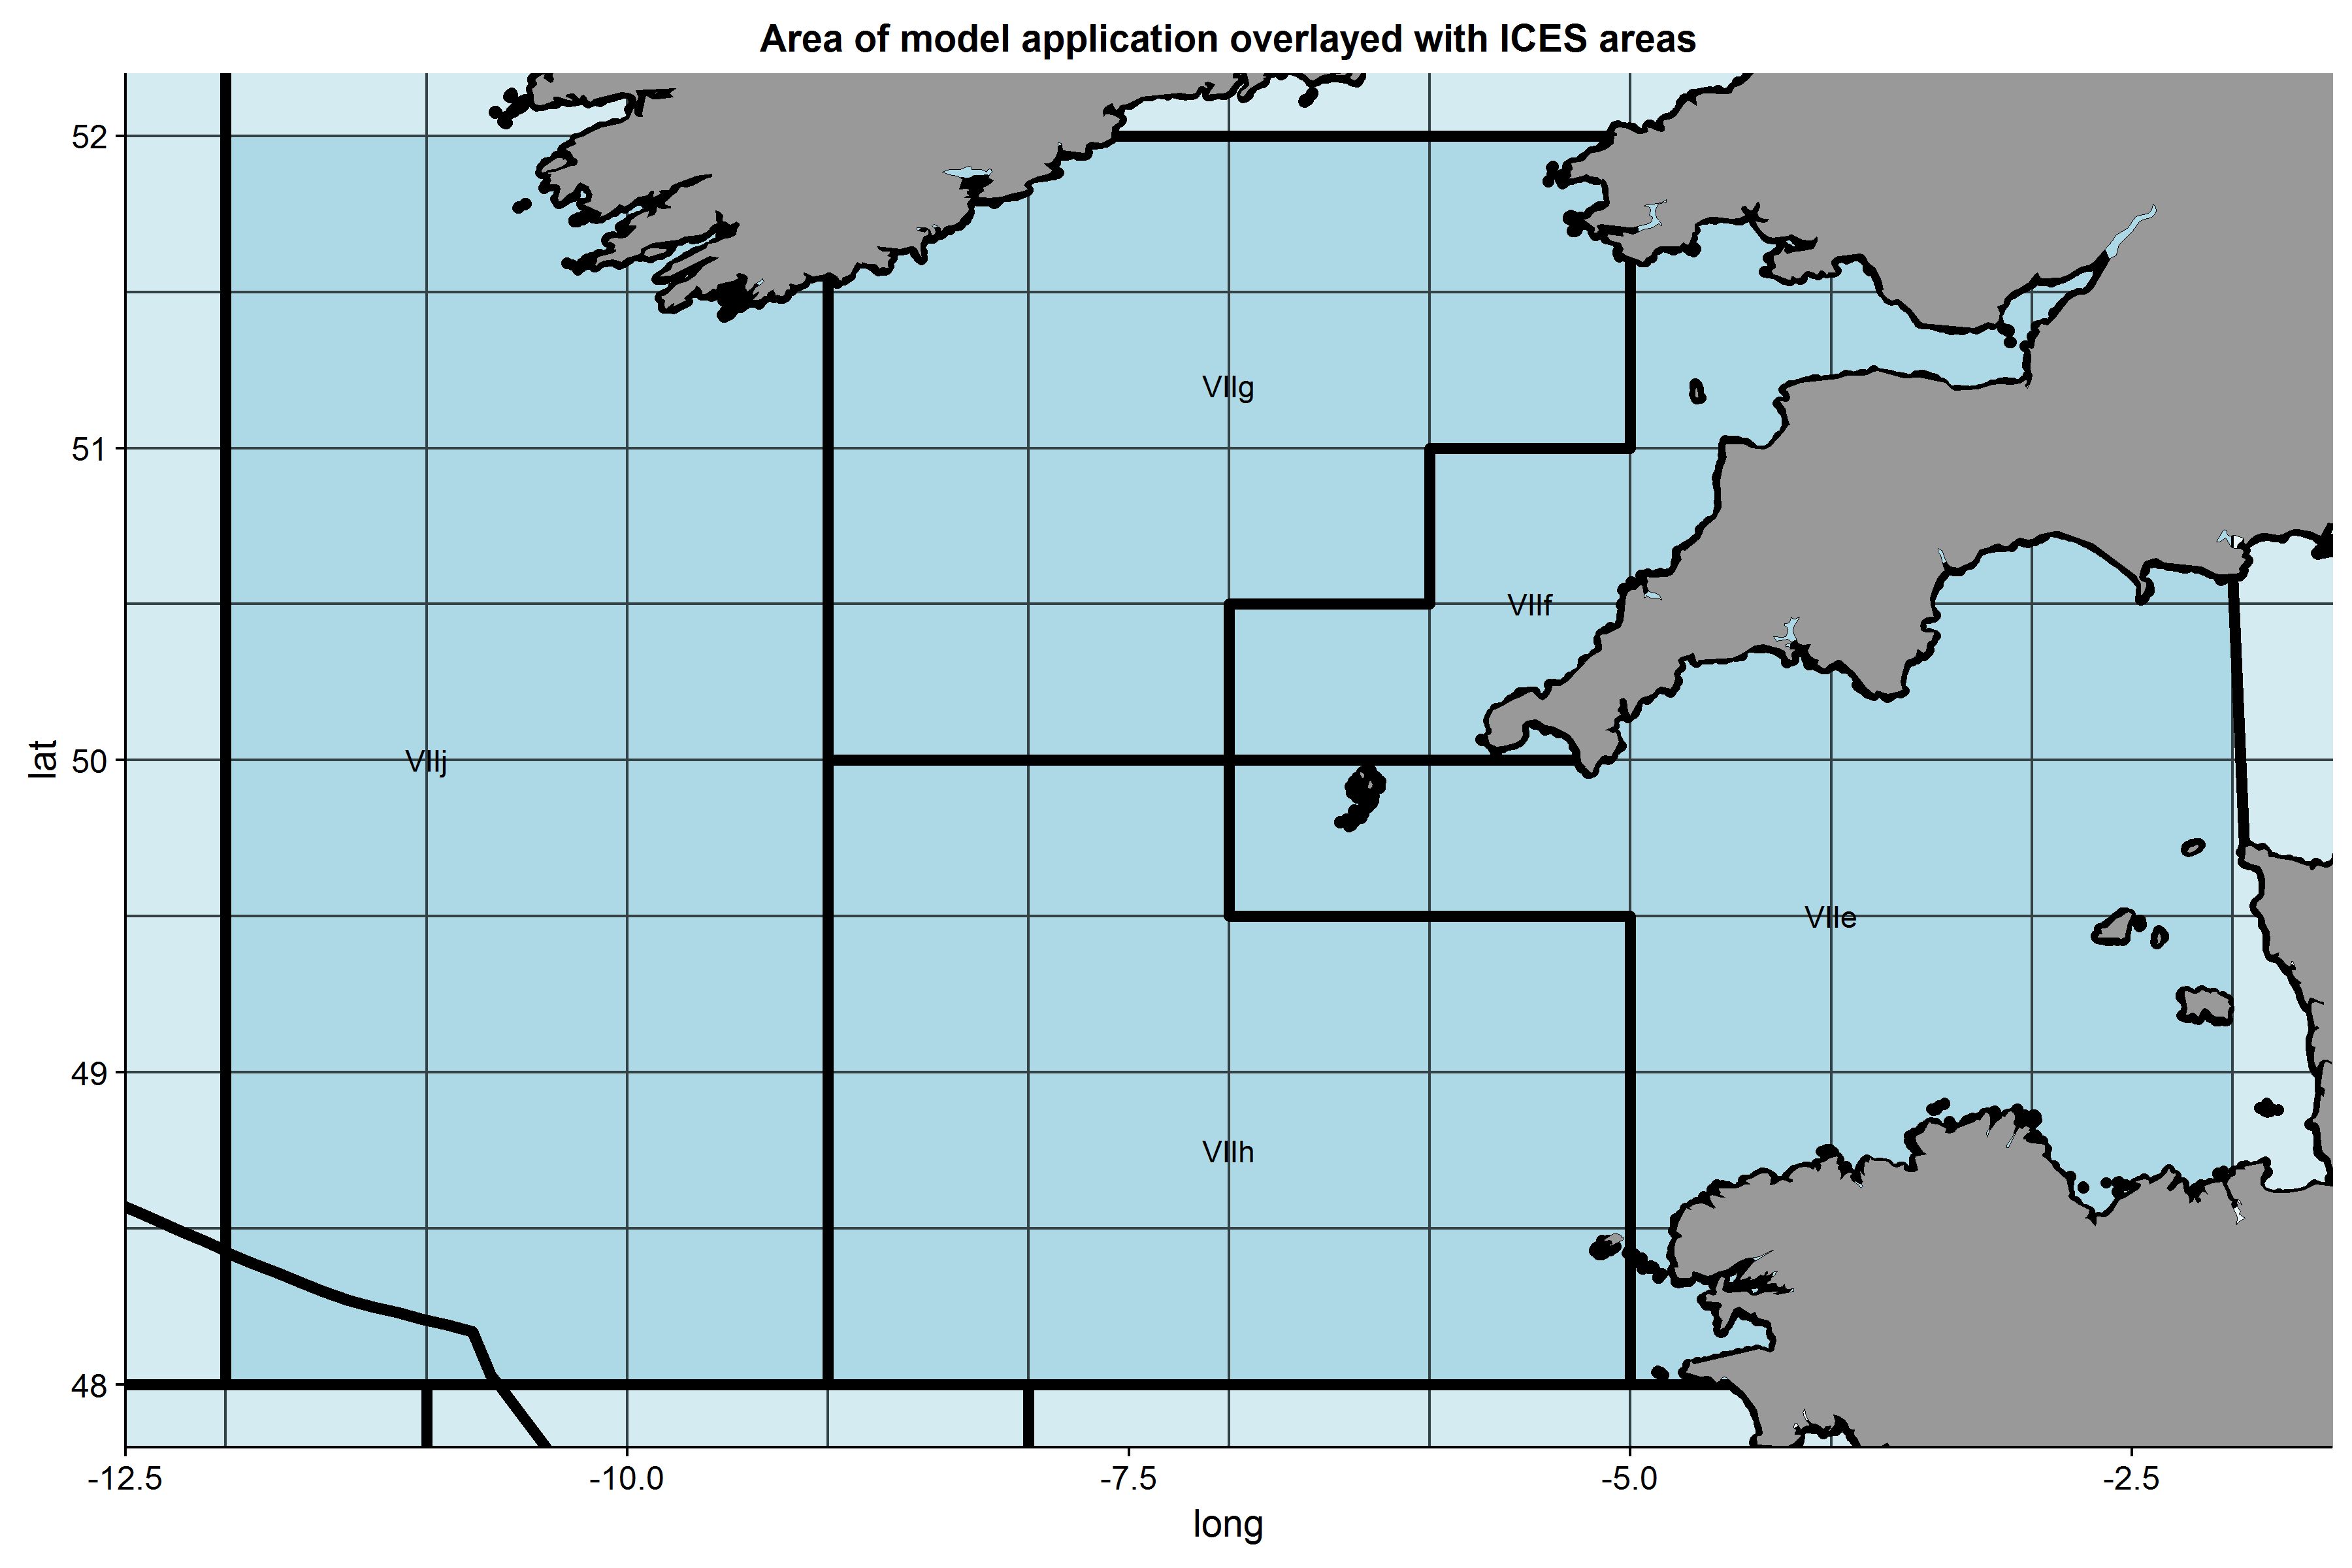
\includegraphics[width=0.5\linewidth]{AreaMap}

\end{frame}

%%%%%%%%%%%%%%%%%%%%%%%%%%%%%%%%%%%%%%%%%%%%%%%%%%%%%%
%%%%%%%%%%%%%%%%%%%%%%%%%%%%%%%%%%%%%%%%%%%%%%%%%%%%%%

\section{Methods}
\subsection{Blah}

\begin{frame}

Four key components:

\begin{enumerate}
	\small
	\setlength\itemsep{2em}

	\item Joint Dynamic Species Distribution Model (JDSDM) able to take
		account of latent (unobserved) drivers which affect species
		distribution and density for one or more species, 
	\item separate modelling of encounter probability and positive catch
		rates (so called 'delta' and 'hurdle' models), 
	\item the use of Gaussian Markov Random Fields (GMRFs) to model the
		variation in probability of occurrence and density as a
		three-dimensional multivariate process (latitude, longitude and
		time) 
	\item set in a mixed modelling framework allowing the incorporation of
		both systematic (fixed) effects and random effects. 

\end{enumerate}

\end{frame}


\begin{frame}{Factor analysis}

	Simple explanation - use simple figures / diagrams
	
	Reduces complexity of the problem - explain trends as a combination of
	factors (latent variables)

	Can provide insight to the community dynamics

	
\end{frame}

\begin{frame}{Gaussian Random Fields}

	Tobler's law - things closer together are more similar.

	Such relationships can provide information for poorly sampled species
	through inference of their relationships

\centering
\includegraphics[width=0.5\linewidth]{SpatialDataAndKnots}

\end{frame}

\begin{frame}{delta-GLMM and covariates}

Surveys often are not coordinated, inconsistent design - need to take account
of these differences.

Can take account of both fixed effects (e.g. gear) and random effects in a
mixed modelling framework.

\centering
\includegraphics[width=0.5\linewidth]{"Suppl - QEstimatesALL"}

	
\end{frame}

%%%%%%%%%%%%%%%%%%%%%%%%%%%%%%%%%%%%%%%%%%%%%%%%%%%%%%%%%%%%%
%%%%%%%%%%%%%%%%%%%%%%%%%%%%%%%%%%%%%%%%%%%%%%%%%%%%%%%%%%%%%

\section{Data}
\subsection{Blah}
\begin{frame}
	
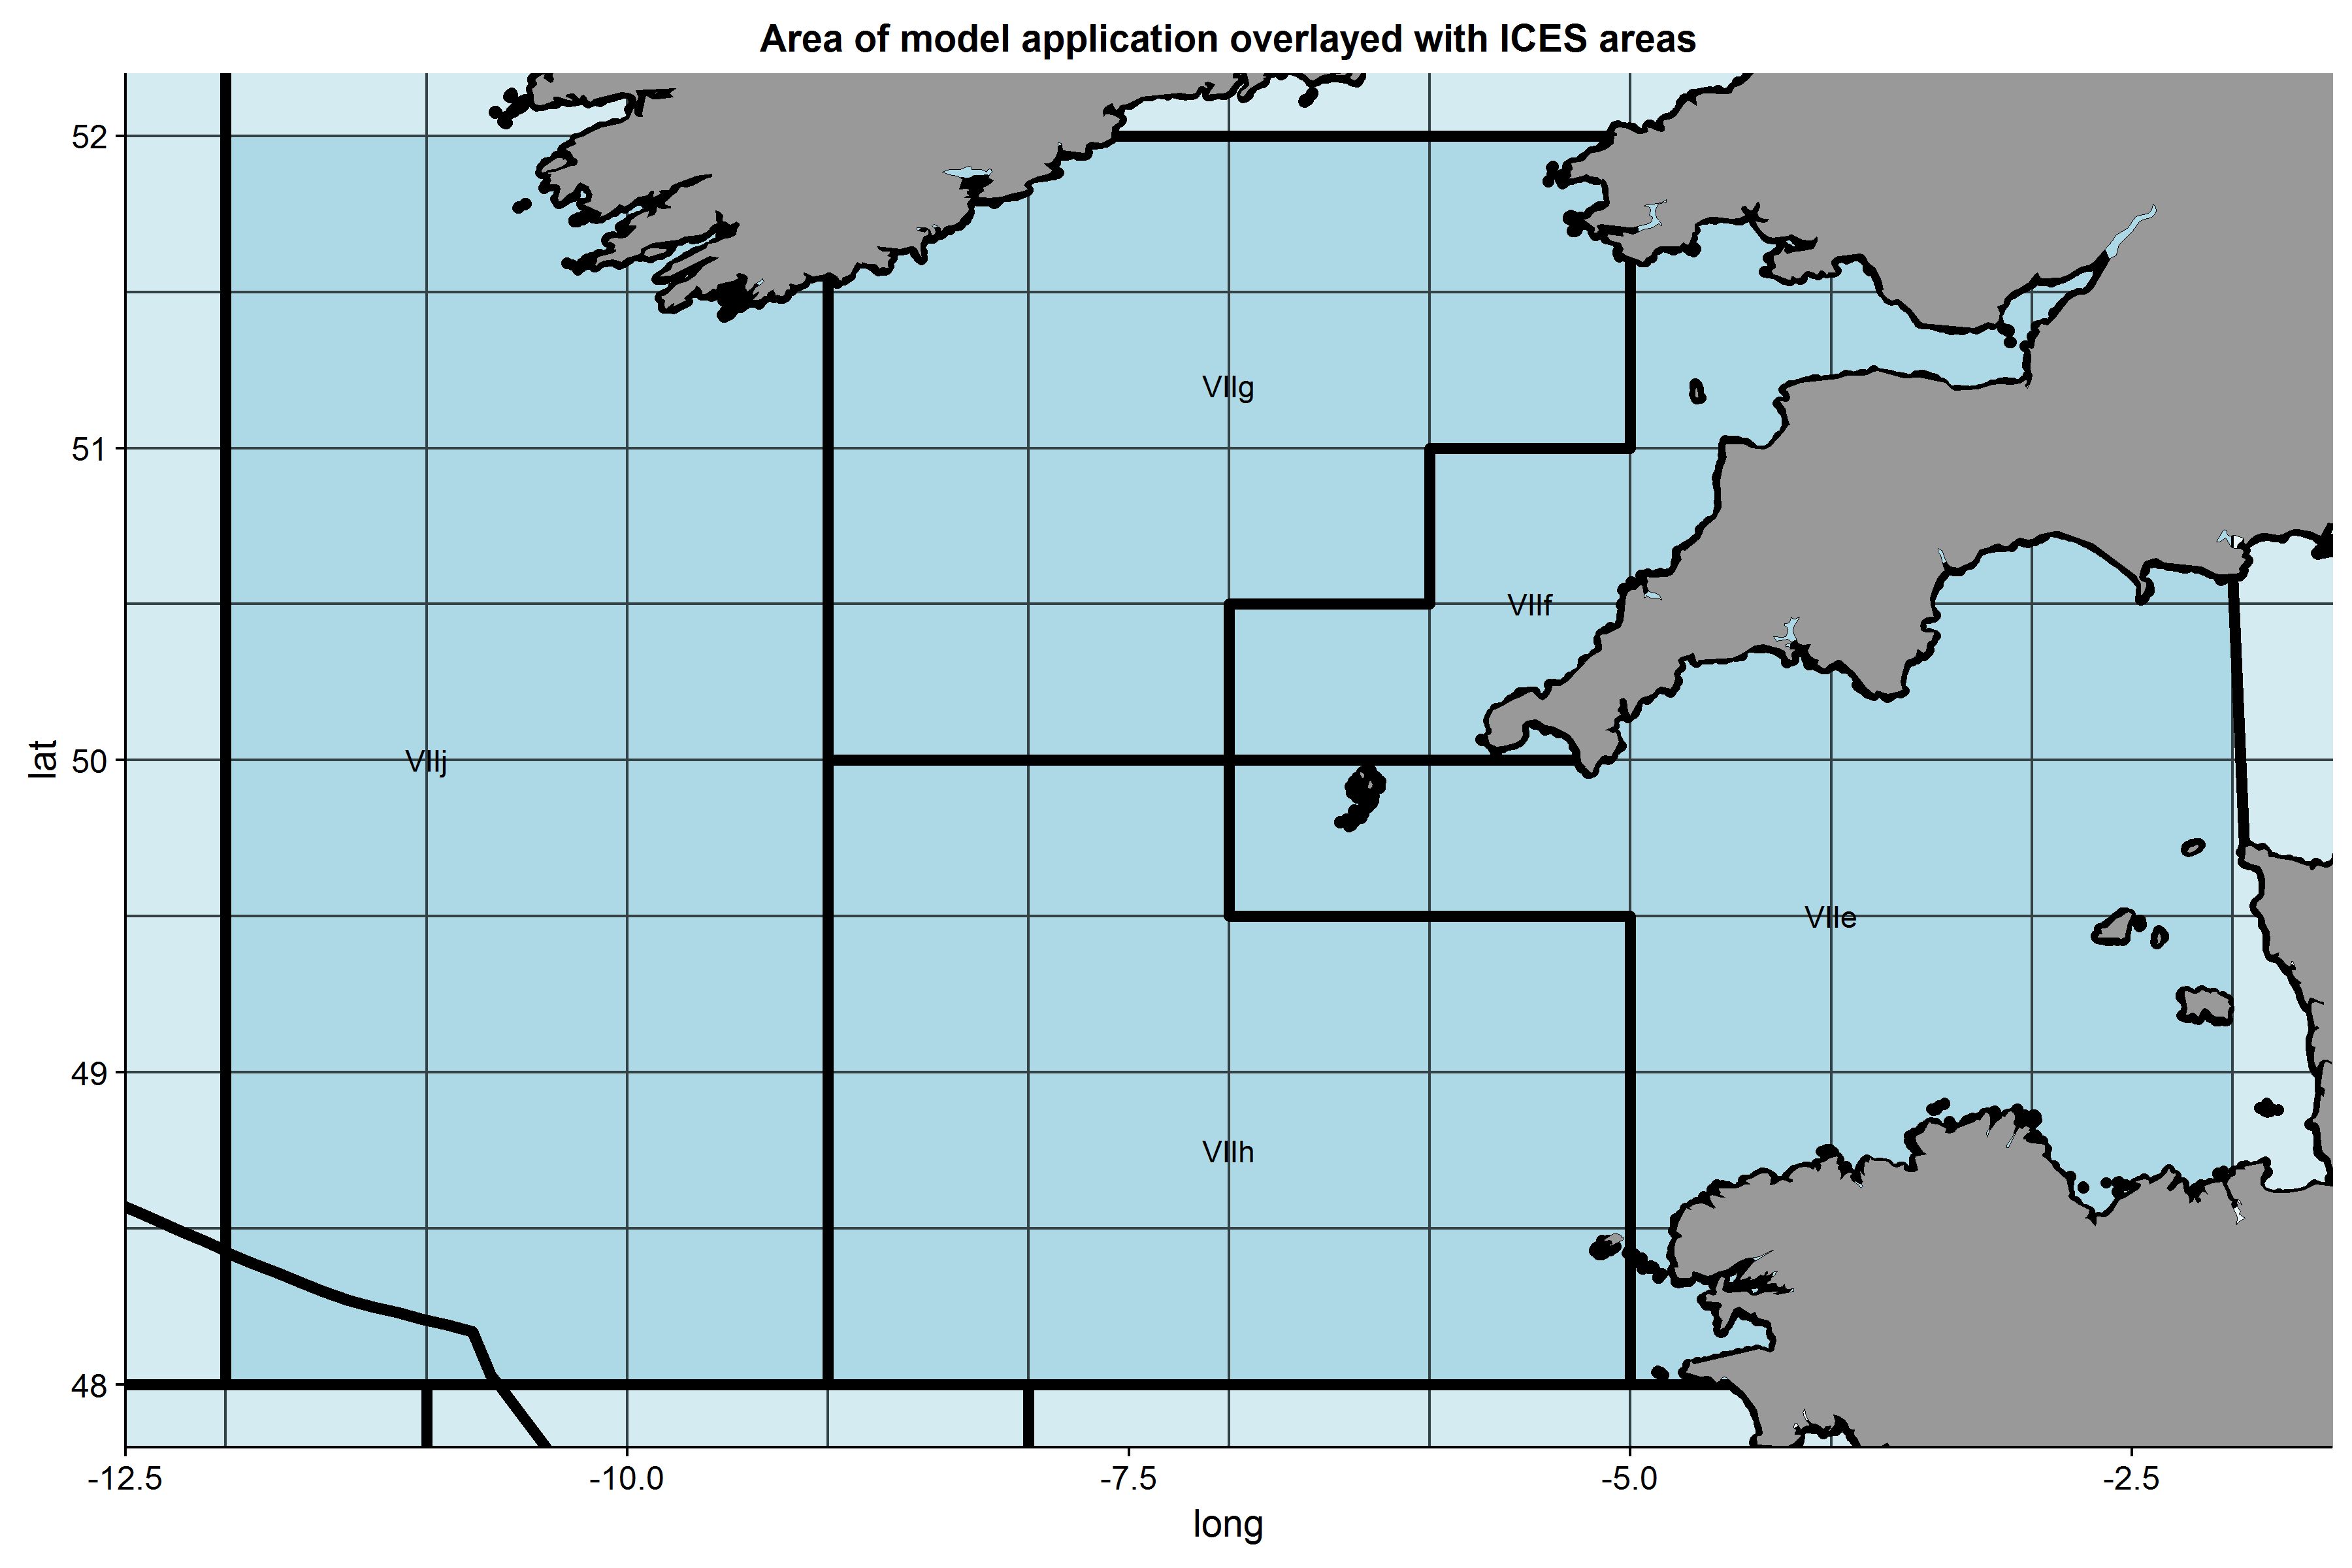
\includegraphics[width=0.5\linewidth]{AreaMap}
\includegraphics[width = 0.1\linewidth]{"Legend"}

\begin{table}[!htb]
	\tiny
	\center
	\begin{tabular}{ p{1cm} p{2cm} p{3cm} p{1cm}}
		\hline
		Species code & Common name              & Species & MCRS (cm) \\
		\hline
		juv          & Juvenile                 & & \\
		adu          & Adult                    & & \\
		\hline
		bud          & Black bellied anglerfish & \textit{Lophius budgessa} & 32* \\
		cod          & Atlantic cod             & \textit{Gadus morhua} & 35 \\
		had          & Atlatic haddock          & \textit{Melanogrammus	aeglefinus} & 30 \\
		hke          & Atlantic hake            & \textit{Merluccius merluccius} & 27 \\
		meg          & Megrim                   & \textit{Lepidorhombus whiffiagonis} & 20\\
		pisc         & White bellied anglerfish & \textit{Lophius piscatorius} & 32* \\
		ple          & European Plaice          & \textit{Pleuronectes platessa} & 27 \\
		sol          & Common sole              & \textit{Solea solea} & 24 \\
		whg          & Atlantic whiting         & \textit{Merlangius merlangus} & 27 \\
		\hline
		\end{tabular}

\end{table}
\end{frame}


\begin{frame}

\begin{table}[!htb]
	\tiny
	\center
	\begin{tabular}{ p{1.5cm} p{3cm} p{2cm} p{1.5cm} }
		\hline
		Survey code    & Name 	& Gear & Temporal extent \\
		\hline
		CEXP / IE-IGFS & Celtic Explorer (IE)   & Otter trawl & 2003 - 2015 \\
		CARLHELMAR     & Carlhelmar (UK)	& Commercial beam trawl & 1989 - 2013 \\
		NWGFS          & North West groundfish survey (UK) & Beam trawl & 1988 - 2015 \\
		Q1SWBEAM       & Quarter 1 south-west beam trawl survey (UK) 	& beam trawl & 2006 - 2015 \\
		Q4SWIBTS       & Quarter 4 south-west international bottom trawl survey (UK) & Otter trawl & 2003 - 2010 \\
		THA2 / EVHOE    & EVHOE survey on Thalasa (FR) & Otter trawl & 1997 - 2015 \\
		WCGFS          & Wstern channel groundfish survey (UK) & Otter
		trawl (Portuguese high headline) & 1982 - 2004 \\
		\hline
	\end{tabular}
\end{table}

\centering
\includegraphics[width=0.5\linewidth]{Survey_effort_by_year-1}

\end{frame}





\section{Findings}
\subsection{Blah}

\begin{frame}{Spatial Encounter correlations}

\centering
\includegraphics[width = 0.7\linewidth]{"Figure 1 - Omega1_Correlations_blank"}
\includegraphics[width = 0.2\linewidth]{"Legend"}

	
\end{frame}

\begin{frame}{Spatial density correlations}

\centering
\includegraphics[width = 0.7\linewidth]{"Figure 1 - Omega2_Correlations_blank"}
\includegraphics[width = 0.2\linewidth]{"Legend"}

\end{frame}

\begin{frame}
	What is driving these associations ?
\end{frame}

\begin{frame}{Spatial factor analysis}

\centering
\includegraphics[width = \linewidth]{"Figure 2 - SpatialFactorLoadingsOmega1"}
\\
\includegraphics[width = \linewidth]{"Figure 2 - SpatialFactorLoadingsOmega2"}
	
\end{frame}

\begin{frame}
        What happens when we consider how they change over time ?	
\end{frame}

\begin{frame}{Spatial factor analysis}

\centering
\includegraphics[width = 0.6\linewidth]{"Suppl - SpatioTempLoadingsEpsilon1"}
	
\end{frame}


\begin{frame}{Spatio-temporal factor loadings - encounter}

\centering
\includegraphics[width = 0.7\linewidth]{"Figure 3 - PCAstyle_Plots_SpatioTempEnc"}
\includegraphics[width = 0.2\linewidth]{"Legend"}

\end{frame}

\begin{frame}{Spatio-temporal factor loadings - density}

\centering
\includegraphics[width = 0.7\linewidth]{"Figure 3 - PCAstyle_Plots_SpatioTempDen"}
\includegraphics[width = 0.2\linewidth]{"Legend"}


\end{frame}

%%%%%%%%%%%%%%%%%%%%%%%%%%%%%%%%%%%%%%%%%%%%%%%%%%%%%%%%%%
%%%%%%%%%%%%%%%%%%%%%%%%%%%%%%%%%%%%%%%%%%%%%%%%%%%%%%%%%%
\section{Implications}
\subsection{Blah}

\begin{frame}{Mixed fisheries}
	
\centering
\includegraphics[width = \linewidth]{"Figure 4 - DensityDifferencesFigureswithCC"}

\end{frame}


\begin{frame}
	Key take home messages
	Whats next etc...
\end{frame}

%%%%%%%%%%%%%%%%%%%%%%%%%%%%%%%%%%%%%%%%%%%%%%%%%%%%%%
\end{document}
%%%%%%%%%%%%%%%%%%%%%%%%%%%%%%%%%%%%%%%%%%%%%%%%%%%%%%
%%%%%%%%%%%%%%%%%%%%%%%%%%%%%%%%%%%%%%%%%%%%%%%%%%%%%%
